\documentclass{standalone}
\usepackage{tikz}
\usetikzlibrary{patterns, positioning}
\usepackage[sfdefault]{ClearSans} %% option 'sfdefault' activates Clear Sans as the default text font
\usepackage[T1]{fontenc}

\begin{document}
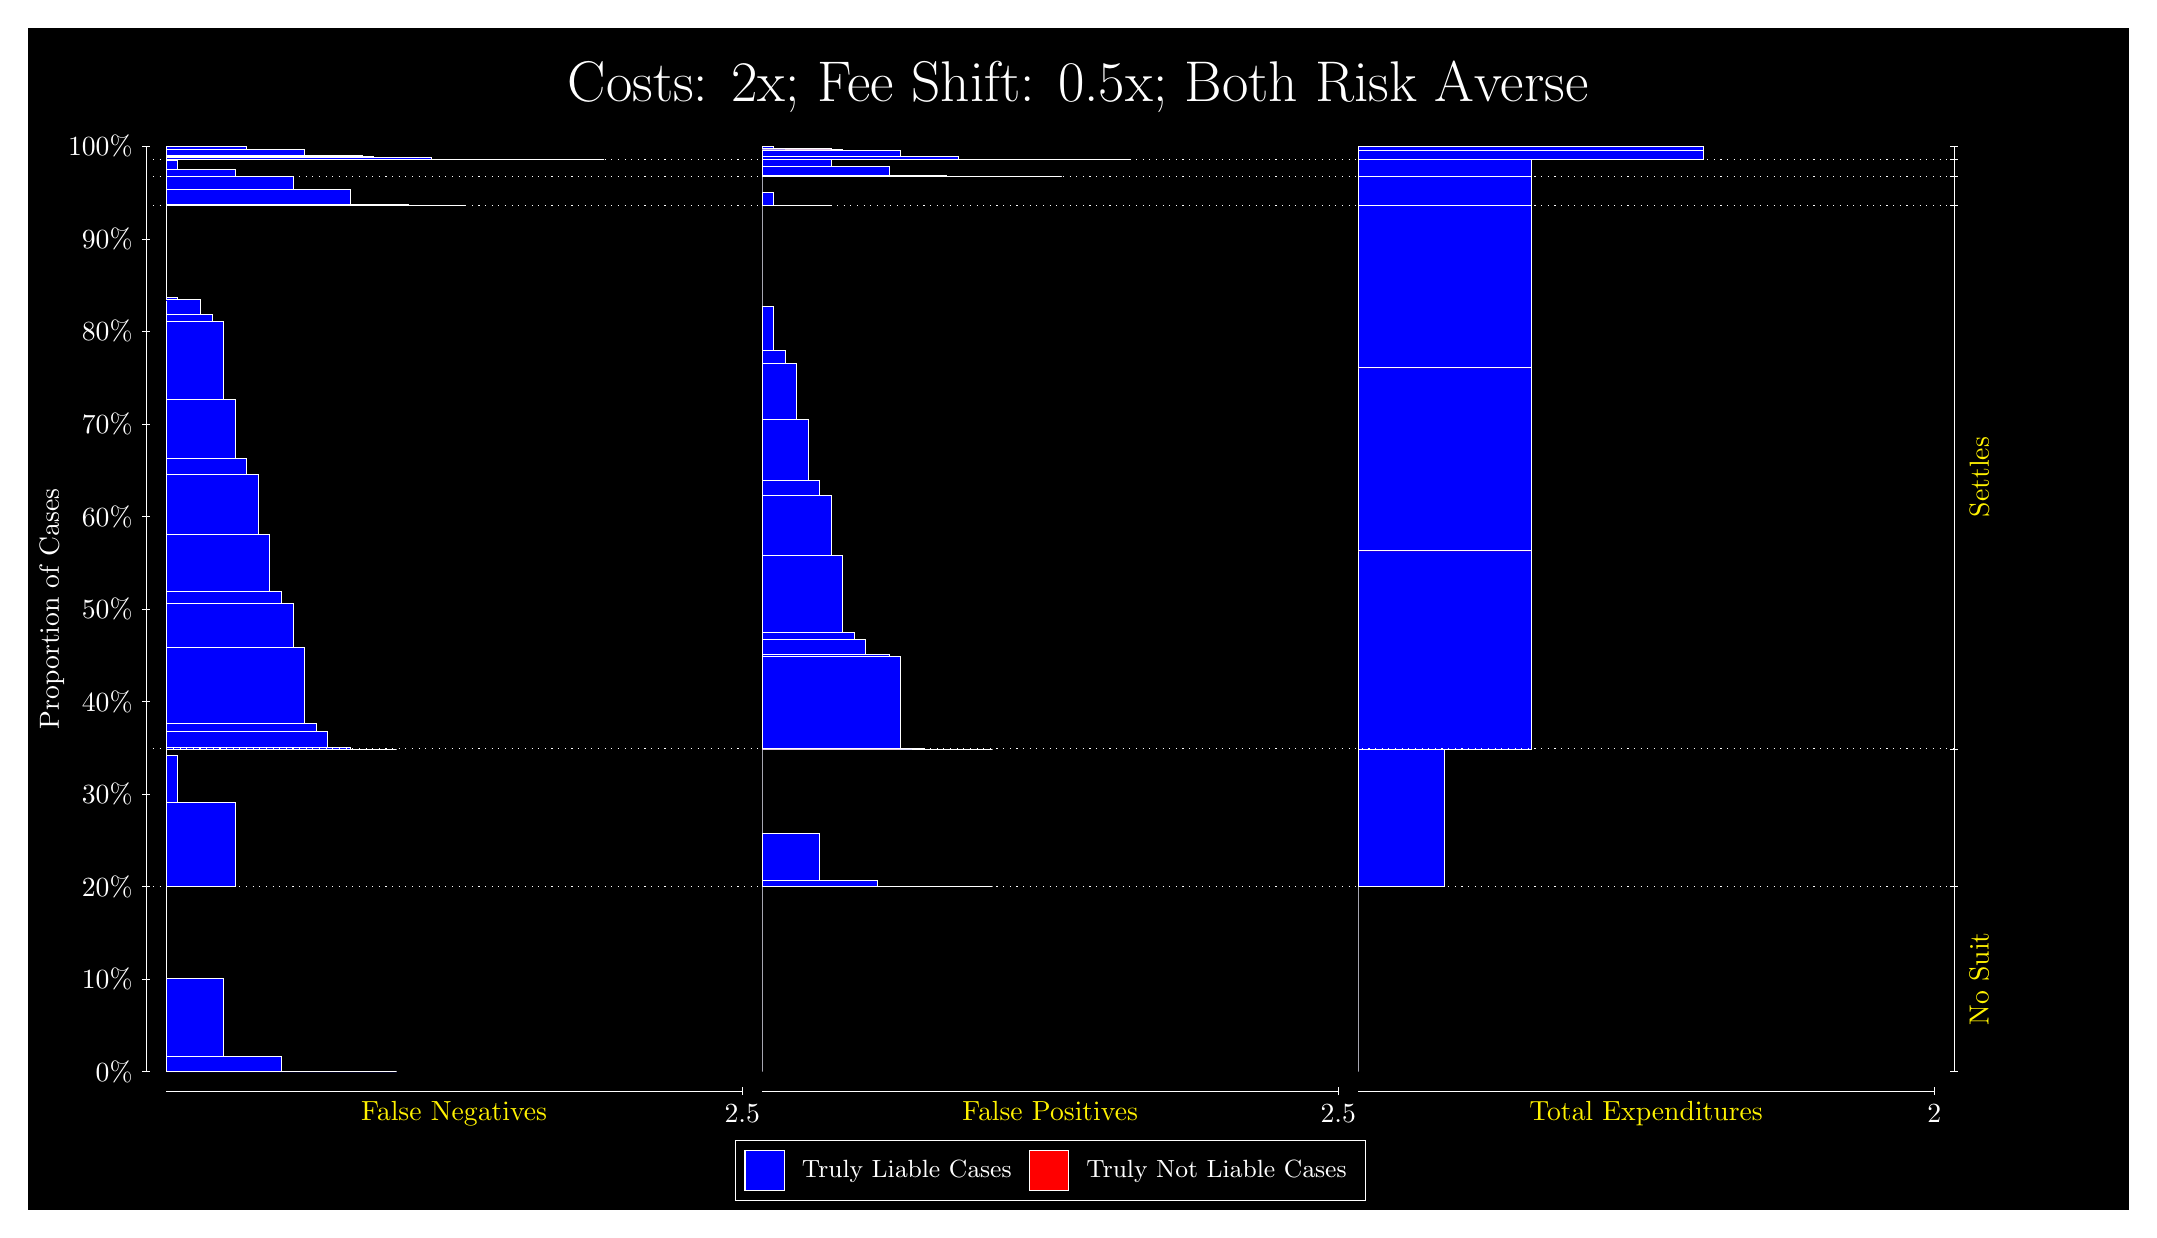
\begin{tikzpicture}
\draw[fill=black] (0,0) rectangle (26.667,15);
\draw[text=white] (0,13.5) rectangle (26.667,15) node[midway] {\huge Costs: 2x; Fee Shift: 0.5x; Both Risk Averse};
\draw[white, very thin] (1.5,1.75) -- (1.5,13.5);
\node[rotate=90, text=white, anchor=center] at (0.3, 7.625) {Proportion of Cases};
\draw[white, very thin] (1.45,1.75) -- (1.55,1.75);
\node[text=white, anchor=east] at (1.45, 1.75) {0\%};
\draw[white, very thin] (1.45,2.925) -- (1.55,2.925);
\node[text=white, anchor=east] at (1.45, 2.925) {10\%};
\draw[white, very thin] (1.45,4.1) -- (1.55,4.1);
\node[text=white, anchor=east] at (1.45, 4.1) {20\%};
\draw[white, very thin] (1.45,5.275) -- (1.55,5.275);
\node[text=white, anchor=east] at (1.45, 5.275) {30\%};
\draw[white, very thin] (1.45,6.45) -- (1.55,6.45);
\node[text=white, anchor=east] at (1.45, 6.45) {40\%};
\draw[white, very thin] (1.45,7.625) -- (1.55,7.625);
\node[text=white, anchor=east] at (1.45, 7.625) {50\%};
\draw[white, very thin] (1.45,8.8) -- (1.55,8.8);
\node[text=white, anchor=east] at (1.45, 8.8) {60\%};
\draw[white, very thin] (1.45,9.975) -- (1.55,9.975);
\node[text=white, anchor=east] at (1.45, 9.975) {70\%};
\draw[white, very thin] (1.45,11.15) -- (1.55,11.15);
\node[text=white, anchor=east] at (1.45, 11.15) {80\%};
\draw[white, very thin] (1.45,12.325) -- (1.55,12.325);
\node[text=white, anchor=east] at (1.45, 12.325) {90\%};
\draw[white, very thin] (1.45,13.5) -- (1.55,13.5);
\node[text=white, anchor=east] at (1.45, 13.5) {100\%};

\draw[white, very thin] (24.457,1.75) -- (24.457,13.5);
\draw[white, very thin] (24.407,1.75) -- (24.507,1.75);
\node[anchor=west] at (24.407, 1.75) {};
\draw[white, very thin] (24.407,4.1018) -- (24.507,4.1018);
\node[anchor=west] at (24.407, 4.1018) {};
\draw[white, very thin] (24.407,5.848) -- (24.507,5.848);
\node[anchor=west] at (24.407, 5.848) {};
\draw[white, very thin] (24.407,12.754) -- (24.507,12.754);
\node[anchor=west] at (24.407, 12.754) {};
\draw[white, very thin] (24.407,13.12) -- (24.507,13.12);
\node[anchor=west] at (24.407, 13.12) {};
\draw[white, very thin] (24.407,13.334) -- (24.507,13.334);
\node[anchor=west] at (24.407, 13.334) {};
\draw[white, very thin] (24.407,13.5) -- (24.507,13.5);
\node[anchor=west] at (24.407, 13.5) {};

\draw[white, very thin, fill=blue] (1.75,1.75) rectangle (4.6775,1.75);
\draw[white, very thin, fill=blue] (1.75,1.75) rectangle (3.9457,1.752);
\draw[white, very thin, fill=blue] (1.75,1.752) rectangle (3.2138,1.9399);
\draw[white, very thin, fill=blue] (1.75,1.9399) rectangle (2.4819,2.9286);
\draw[white, very thin, fill=red] (1.75,2.9286) rectangle (1.75,2.9286);
\draw[white, very thin, fill=blue] (1.75,2.9286) rectangle (1.75,4.1018);
\draw[white, very thin, fill=blue] (1.75,4.1018) rectangle (2.6283,5.1682);
\draw[white, very thin, fill=blue] (1.75,5.1682) rectangle (1.8964,5.7659);
\draw[white, very thin, fill=red] (1.75,5.7659) rectangle (1.75,5.7659);
\draw[white, very thin, fill=blue] (1.75,5.7659) rectangle (1.75,5.848);
\draw[white, very thin, fill=blue] (1.75,5.848) rectangle (4.6775,5.848);
\draw[white, very thin, fill=blue] (1.75,5.848) rectangle (4.3848,5.8481);
\draw[white, very thin, fill=blue] (1.75,5.8481) rectangle (4.092,5.8674);
\draw[white, very thin, fill=blue] (1.75,5.8674) rectangle (3.9457,5.8679);
\draw[white, very thin, fill=blue] (1.75,5.8679) rectangle (3.7993,6.0761);
\draw[white, very thin, fill=blue] (1.75,6.0761) rectangle (3.6529,6.1687);
\draw[white, very thin, fill=blue] (1.75,6.1687) rectangle (3.5065,7.1325);
\draw[white, very thin, fill=blue] (1.75,7.1325) rectangle (3.3602,7.6926);
\draw[white, very thin, fill=blue] (1.75,7.6926) rectangle (3.2138,7.8541);
\draw[white, very thin, fill=blue] (1.75,7.8541) rectangle (3.0674,8.5667);
\draw[white, very thin, fill=blue] (1.75,8.5667) rectangle (2.921,9.3406);
\draw[white, very thin, fill=blue] (1.75,9.3406) rectangle (2.7746,9.5331);
\draw[white, very thin, fill=blue] (1.75,9.5331) rectangle (2.6283,10.289);
\draw[white, very thin, fill=blue] (1.75,10.289) rectangle (2.4819,11.277);
\draw[white, very thin, fill=blue] (1.75,11.277) rectangle (2.3355,11.365);
\draw[white, very thin, fill=blue] (1.75,11.365) rectangle (2.1891,11.552);
\draw[white, very thin, fill=blue] (1.75,11.552) rectangle (2.0428,11.554);
\draw[white, very thin, fill=blue] (1.75,11.554) rectangle (1.8964,11.579);
\draw[white, very thin, fill=red] (1.75,11.579) rectangle (1.75,11.579);
\draw[white, very thin, fill=blue] (1.75,11.579) rectangle (1.75,12.754);
\draw[white, very thin, fill=blue] (1.75,12.754) rectangle (5.5558,12.754);
\draw[white, very thin, fill=blue] (1.75,12.754) rectangle (4.8239,12.758);
\draw[white, very thin, fill=blue] (1.75,12.758) rectangle (4.092,12.959);
\draw[white, very thin, fill=blue] (1.75,12.959) rectangle (3.3602,13.118);
\draw[white, very thin, fill=blue] (1.75,13.118) rectangle (2.6283,13.12);
\draw[white, very thin, fill=red] (1.75,13.12) rectangle (1.75,13.12);
\draw[white, very thin, fill=blue] (1.75,13.12) rectangle (2.6283,13.21);
\draw[white, very thin, fill=blue] (1.75,13.21) rectangle (1.8964,13.327);
\draw[white, very thin, fill=red] (1.75,13.327) rectangle (1.75,13.327);
\draw[white, very thin, fill=blue] (1.75,13.327) rectangle (1.75,13.334);
\draw[white, very thin, fill=blue] (1.75,13.334) rectangle (7.3123,13.334);
\draw[white, very thin, fill=blue] (1.75,13.334) rectangle (6.5805,13.334);
\draw[white, very thin, fill=blue] (1.75,13.334) rectangle (5.8486,13.338);
\draw[white, very thin, fill=blue] (1.75,13.338) rectangle (5.7022,13.338);
\draw[white, very thin, fill=blue] (1.75,13.338) rectangle (5.1167,13.364);
\draw[white, very thin, fill=blue] (1.75,13.364) rectangle (4.9703,13.364);
\draw[white, very thin, fill=blue] (1.75,13.364) rectangle (4.3848,13.371);
\draw[white, very thin, fill=blue] (1.75,13.371) rectangle (4.2384,13.384);
\draw[white, very thin, fill=blue] (1.75,13.384) rectangle (3.6529,13.384);
\draw[white, very thin, fill=blue] (1.75,13.384) rectangle (3.5065,13.46);
\draw[white, very thin, fill=blue] (1.75,13.46) rectangle (2.921,13.46);
\draw[white, very thin, fill=blue] (1.75,13.46) rectangle (2.7746,13.498);
\draw[white, very thin, fill=blue] (1.75,13.498) rectangle (2.0428,13.5);
\draw[white, very thin, fill=red] (1.75,13.5) rectangle (1.75,13.5);
\draw[white, very thin, fill=blue] (1.75,13.5) rectangle (1.75,13.5);
\draw[white, very thin, fill=red] (9.3189,1.75) rectangle (9.3189,1.75);
\draw[white, very thin, fill=blue] (9.3189,1.75) rectangle (9.3189,4.1018);
\draw[white, very thin, fill=red] (9.3189,4.1018) rectangle (12.246,4.1018);
\draw[white, very thin, fill=blue] (9.3189,4.1018) rectangle (12.246,4.1018);
\draw[white, very thin, fill=blue] (9.3189,4.1018) rectangle (11.515,4.1019);
\draw[white, very thin, fill=blue] (9.3189,4.1019) rectangle (10.783,4.1838);
\draw[white, very thin, fill=blue] (9.3189,4.1838) rectangle (10.051,4.7815);
\draw[white, very thin, fill=blue] (9.3189,4.7815) rectangle (9.3189,5.848);
\draw[white, very thin, fill=red] (9.3189,5.848) rectangle (12.246,5.848);
\draw[white, very thin, fill=blue] (9.3189,5.848) rectangle (12.246,5.848);
\draw[white, very thin, fill=red] (9.3189,5.848) rectangle (11.954,5.848);
\draw[white, very thin, fill=blue] (9.3189,5.848) rectangle (11.954,5.848);
\draw[white, very thin, fill=red] (9.3189,5.848) rectangle (11.661,5.848);
\draw[white, very thin, fill=blue] (9.3189,5.848) rectangle (11.661,5.848);
\draw[white, very thin, fill=blue] (9.3189,5.848) rectangle (11.515,5.848);
\draw[white, very thin, fill=red] (9.3189,5.848) rectangle (11.368,5.848);
\draw[white, very thin, fill=blue] (9.3189,5.848) rectangle (11.368,5.8499);
\draw[white, very thin, fill=blue] (9.3189,5.8499) rectangle (11.222,5.85);
\draw[white, very thin, fill=red] (9.3189,5.85) rectangle (11.075,5.85);
\draw[white, very thin, fill=blue] (9.3189,5.85) rectangle (11.075,7.0231);
\draw[white, very thin, fill=blue] (9.3189,7.0231) rectangle (10.929,7.048);
\draw[white, very thin, fill=blue] (9.3189,7.048) rectangle (10.783,7.0498);
\draw[white, very thin, fill=blue] (9.3189,7.0498) rectangle (10.636,7.2367);
\draw[white, very thin, fill=blue] (9.3189,7.2367) rectangle (10.49,7.3248);
\draw[white, very thin, fill=blue] (9.3189,7.3248) rectangle (10.344,8.3126);
\draw[white, very thin, fill=blue] (9.3189,8.3126) rectangle (10.197,9.0686);
\draw[white, very thin, fill=blue] (9.3189,9.0686) rectangle (10.051,9.2611);
\draw[white, very thin, fill=blue] (9.3189,9.2611) rectangle (9.9044,10.035);
\draw[white, very thin, fill=blue] (9.3189,10.035) rectangle (9.758,10.748);
\draw[white, very thin, fill=blue] (9.3189,10.748) rectangle (9.6116,10.909);
\draw[white, very thin, fill=blue] (9.3189,10.909) rectangle (9.4652,11.469);
\draw[white, very thin, fill=blue] (9.3189,11.469) rectangle (9.3189,12.754);
\draw[white, very thin, fill=red] (9.3189,12.754) rectangle (10.197,12.754);
\draw[white, very thin, fill=blue] (9.3189,12.754) rectangle (10.197,12.756);
\draw[white, very thin, fill=blue] (9.3189,12.756) rectangle (9.4652,12.914);
\draw[white, very thin, fill=blue] (9.3189,12.914) rectangle (9.3189,13.12);
\draw[white, very thin, fill=red] (9.3189,13.12) rectangle (13.125,13.12);
\draw[white, very thin, fill=blue] (9.3189,13.12) rectangle (13.125,13.12);
\draw[white, very thin, fill=blue] (9.3189,13.12) rectangle (12.393,13.12);
\draw[white, very thin, fill=blue] (9.3189,13.12) rectangle (11.661,13.127);
\draw[white, very thin, fill=blue] (9.3189,13.127) rectangle (10.929,13.244);
\draw[white, very thin, fill=blue] (9.3189,13.244) rectangle (10.197,13.334);
\draw[white, very thin, fill=red] (9.3189,13.334) rectangle (14.003,13.334);
\draw[white, very thin, fill=blue] (9.3189,13.334) rectangle (14.003,13.334);
\draw[white, very thin, fill=red] (9.3189,13.334) rectangle (13.271,13.334);
\draw[white, very thin, fill=blue] (9.3189,13.334) rectangle (13.271,13.334);
\draw[white, very thin, fill=red] (9.3189,13.334) rectangle (12.539,13.334);
\draw[white, very thin, fill=blue] (9.3189,13.334) rectangle (12.539,13.336);
\draw[white, very thin, fill=blue] (9.3189,13.336) rectangle (11.807,13.374);
\draw[white, very thin, fill=red] (9.3189,13.374) rectangle (11.807,13.374);
\draw[white, very thin, fill=blue] (9.3189,13.374) rectangle (11.807,13.374);
\draw[white, very thin, fill=red] (9.3189,13.374) rectangle (11.661,13.374);
\draw[white, very thin, fill=blue] (9.3189,13.374) rectangle (11.661,13.374);
\draw[white, very thin, fill=blue] (9.3189,13.374) rectangle (11.075,13.45);
\draw[white, very thin, fill=blue] (9.3189,13.45) rectangle (11.075,13.45);
\draw[white, very thin, fill=red] (9.3189,13.45) rectangle (10.929,13.45);
\draw[white, very thin, fill=blue] (9.3189,13.45) rectangle (10.929,13.45);
\draw[white, very thin, fill=blue] (9.3189,13.45) rectangle (10.344,13.457);
\draw[white, very thin, fill=blue] (9.3189,13.457) rectangle (10.344,13.463);
\draw[white, very thin, fill=blue] (9.3189,13.463) rectangle (10.197,13.47);
\draw[white, very thin, fill=red] (9.3189,13.47) rectangle (10.197,13.47);
\draw[white, very thin, fill=blue] (9.3189,13.47) rectangle (10.197,13.47);
\draw[white, very thin, fill=blue] (9.3189,13.47) rectangle (9.6116,13.47);
\draw[white, very thin, fill=blue] (9.3189,13.47) rectangle (9.6116,13.47);
\draw[white, very thin, fill=blue] (9.3189,13.47) rectangle (9.4652,13.496);
\draw[white, very thin, fill=blue] (9.3189,13.496) rectangle (9.4652,13.496);
\draw[white, very thin, fill=blue] (9.3189,13.496) rectangle (9.3189,13.5);
\draw[white, very thin, fill=red] (16.888,1.75) rectangle (16.888,1.75);
\draw[white, very thin, fill=blue] (16.888,1.75) rectangle (16.888,4.1018);
\draw[white, very thin, fill=red] (16.888,4.1018) rectangle (17.986,4.1018);
\draw[white, very thin, fill=blue] (16.888,4.1018) rectangle (17.986,5.848);
\draw[white, very thin, fill=red] (16.888,5.848) rectangle (19.083,5.848);
\draw[white, very thin, fill=blue] (16.888,5.848) rectangle (19.083,8.3663);
\draw[white, very thin, fill=red] (16.888,8.3663) rectangle (19.083,8.3663);
\draw[white, very thin, fill=blue] (16.888,8.3663) rectangle (19.083,10.689);
\draw[white, very thin, fill=red] (16.888,10.689) rectangle (19.083,10.689);
\draw[white, very thin, fill=blue] (16.888,10.689) rectangle (19.083,12.754);
\draw[white, very thin, fill=red] (16.888,12.754) rectangle (19.083,12.754);
\draw[white, very thin, fill=blue] (16.888,12.754) rectangle (19.083,13.12);
\draw[white, very thin, fill=red] (16.888,13.12) rectangle (19.083,13.12);
\draw[white, very thin, fill=blue] (16.888,13.12) rectangle (19.083,13.334);
\draw[white, very thin, fill=red] (16.888,13.334) rectangle (21.279,13.334);
\draw[white, very thin, fill=blue] (16.888,13.334) rectangle (21.279,13.456);
\draw[white, very thin, fill=red] (16.888,13.456) rectangle (21.279,13.456);
\draw[white, very thin, fill=blue] (16.888,13.456) rectangle (21.279,13.5);
\draw[white, dotted] (1.5,4.1018) -- (24.457,4.1018);
\draw[white, dotted] (1.5,5.848) -- (24.457,5.848);
\draw[white, dotted] (1.5,12.754) -- (24.457,12.754);
\draw[white, dotted] (1.5,13.12) -- (24.457,13.12);
\draw[white, dotted] (1.5,13.334) -- (24.457,13.334);
\draw[white, very thin] (1.75,1.5) -- (9.0689,1.5);
\node[text=yellow, anchor=north] at (5.4094, 1.5) {False Negatives};
\draw[white, very thin] (9.0689,1.45) -- (9.0689,1.55);
\node[text=white, anchor=north] at (9.0689, 1.45) {2.5};

\draw[white, very thin] (9.3189,1.5) -- (16.638,1.5);
\node[text=yellow, anchor=north] at (12.978, 1.5) {False Positives};
\draw[white, very thin] (16.638,1.45) -- (16.638,1.55);
\node[text=white, anchor=north] at (16.638, 1.45) {2.5};

\draw[white, very thin] (16.888,1.5) -- (24.207,1.5);
\node[text=yellow, anchor=north] at (20.547, 1.5) {Total Expenditures};
\draw[white, very thin] (24.207,1.45) -- (24.207,1.55);
\node[text=white, anchor=north] at (24.207, 1.45) {2};

\node[text=yellow, centered, rotate=90] at (24.777, 2.9259) {No Suit};

\node[text=yellow, centered, rotate=90] at (24.777, 9.3009) {Settles};




\draw (12.978300999999998,1.5) node[draw=none] (baseCoordinate) {};
\begin{scope}[align=center]
        \matrix[scale=0.5, draw=white, below=0.5cm of baseCoordinate, nodes={draw}, column sep=0.1cm]{
            \node[rectangle, draw, minimum width=0.5cm, minimum height=0.5cm, fill=blue] {}; &
            \node[draw=none, font=\small, text=white] (B) {Truly Liable Cases}; &
            \node[rectangle, draw, minimum width=0.5cm, minimum height=0.5cm, fill=red] {}; &
            \node[draw=none, font=\small, text=white] (B) {Truly Not Liable Cases}; \\
            };
\end{scope}

\end{tikzpicture}
\end{document}